\section{Magnetic sectors and the spin lower bound}
\label{sec:magnetic}

Throughout this section, fix \(b>0\) with \(a=a(b)>0\).
We prove the converse to Proposition~\ref{prop:spin-upper}.

\begin{proposition}[Magnetic lower bound]\label{prop:spin-lower}
For the prescribed free-box correlation,
\[
 \liminf_{n\to\infty}\frac{\log C_b(n)}{\log n}
       \ge -\frac{2\pi}{a}.
\]
In particular, \(m(b)=0\).
\end{proposition}

Convergence of ordinary height observations does not by itself compare
partition functions in different winding sectors. We make that comparison
by adding confining observations on each of finitely many scales. Local
Gaussian limits then control guarded bond restorations, and an exact
finite expansion bounds the accumulated error. The high-law inputs are
Theorems~\ref{thm:mixed-limits} and~\ref{thm:pin-interaction} and
Lemma~\ref{lem:restoration}, already proved for the Skellam weights.
The real Gaussian localization estimates used below are the unchanged
ones in \Bcite{an:gaussian-localization}.

\subsection{A localized magnetic sector}

Use coordinates divided by \(n\), so the sources are \(0,e_1\).
Take the outer box sufficiently large that its boundary is well outside
\([-8,8]^2\) in these coordinates. There is a real multivalued function
\(v\), with periods \(2\pi,-2\pi\) at the two sources, which equals a
signed polar angle plus a smooth function near each source and has a
single-valued lift equal to zero outside \([-2,2]^2\). Indeed, the
difference of the two angles has zero period on an outer annulus;
multiply its lift there by a cutoff. Choose bounded-value branches,
with bounded integer jumps. Whenever a local chart is changed, apply
the same integer gauge to the lattice height and to \(v\).

Fix a large microscopic length \(m_*\). Choose \(q\) so that
\[
                 m_*\le 2^{-q}n\le 2m_*,
\]
and remove the dual height vertices in two open squares of half-side
\(2^{-q}\) about the sources, rounding their faces to lattice divisions.
The new inner walls are free. The prescribed connection still has the
two indicated periods in this punctured graph. Below, all observations
are outside the holes and are contained in charts missing the sources.

Let \(B\) be a collection of box averages, to be specified shortly.
Add the observation factor
\begin{equation}\label{eq:magnetic-mass}
 \exp\left\{-\frac12\norm{Bh-Bv}^2\right\}
\end{equation}
in the shifted sector and use target zero in the centered sector.
Equivalently, average the single-valued deviation in each chart.
The two targets and their connection can be chosen zero on a common
outer terminal region. Lemma~\ref{lem:comparisons} shows that adding
\eqref{eq:magnetic-mass} decreases the shifted-to-centered ratio:
in enlarged affine coordinates the new coordinates are \(Bh-Bv\),
versus \(Bh\) on the parallel centered lattice, and we are adding a
positive quadratic form. No integer-valued assumption on \(v\) is used.

Here is the geometry, including the uniformity needed later. First
choose a sufficiently large dyadic integer \(M\), and then a large
dyadic integer \(R\). There is a face-connected tessellation by regular
tiles and one unprocessed exterior object with the following properties.
\begin{enumerate}[label=(\roman*),leftmargin=*]
\item Away from outer termination, tile size is comparable to distance
to the nearer source divided by \(M\), with distance capped at a fixed
constant away from the sources. Each tile contains mass cells whose
side lengths are comparable to its size divided by \(R\).
\item Patches of every fixed tile-radius used below have a bounded
number of tiles, local charts missing the sources, and comparable
mass-cell sizes. Their pre-pin components, including after local bond
deletions, have the mixed geometry of Theorem~\ref{thm:mixed-limits}.
Guards and cores are unions of tiles; their intervening collars have
width comparable to \(R\) in mass-cell units. Mass cells do not cross
a guard or a tile cut.
\item There are at most \(C_M(1+\log n)\) processed tiles and uniformly
bounded face-graph degrees. On each fixed-radius patch, a target lift
has bounded magnitude and bounded sampled gradient energy, uniformly
in \(R,n\). Its vector of mass-cell averages has norm at most a fixed
polynomial in \(R\).
\item The exterior object starts beyond the support of the target,
contains the remaining graph up to the outer height pin, and is never
processed. An ordinary continuation of the local tessellation and
of the mass cells is retained through a wide collar of its inner
boundary. Local patches use this continuation and stay far from the
outer pin. For dependency counting only, tiles attached to the
exterior may be joined through one terminal node of degree bounded
in terms of \(M\); local distances never use this shortcut.
\end{enumerate}

To construct the tessellation, divide the sup-norm neighborhood of
radius \(1/4\) of each source into square rings with successive radii
in ratio two, down to its hole. Subdivide a ring into squares of side
its inner radius divided by \(M\); use a matching uniform grid in the
remaining bounded region. At subdivision junctions insert small
trimmed square tiles, with side a fixed fraction of the shortest
incident side. Clip at the holes when necessary. Thus point contacts
do not join components, and incident sectors which must be joined
have a face, rather than an opposite-only junction. This is the
geometry of \Bcite{an:geometry}. Subdivide all tiles and trimmed
parts into rectangular mass cells of the stated size, with compatible
face subdivisions. Rounded coordinates retain the same adjacencies
when \(m_*\) is large enough.

Choose the fixed patch, guard, skip, and enlargement radii first, and
take \(M\) larger than all of them. After rescaling by the local ring
radius, the patches and their possible local deletions range over
finitely many shapes, up to bounded lattice rounding. Here is why
this covers every integer \(n\), not just dyadic separations.
In primary lattice units the logical ring radii are \(r_j=n2^{-j}\),
stopped with \(m_*\le r_q<2m_*\). Round each shared logical face
once to a dual-lattice division, and reuse it on both sides.
Its displacement is \(O(1)\). A fixed-radius patch spans only
boundedly many neighboring ring scales, so its ideal normalized
shape and deletion pattern belong to finite lists. Its mesh
and face-rounding errors in mass-cell units are at most
\[
                         \frac{C_M R}{r_j}
                                  \le \frac{C_M R}{m_*}.
\]
For large \(m_*\), all widths, incidences, and collars are preserved.

The targets also range over compact smooth families. Near a
source \(z_0\), after scaling by \(\rho_j=r_j/n\), a local lift
has the form \(\pm\arg z+g(z_0+\rho_jz)\), with \(g\) smooth
and \(0<\rho_j\le1/4\). Adjoining \(\rho=0\) closes this
family in the required smooth norms; finitely many angle
charts suffice. The outer patches have fixed smooth families,
and bounded integer chart changes add finitely many choices.
Sampled cell averages converge uniformly on these compact sets.
If a common refinement threshold failed at fixed \(M,R\), a
sequence of failing patches with mesh tending to zero would
have a subsequence with one ideal shape and deletion pattern
and a convergent target. The admissibly rounded high-law and
real Gaussian limits on that subsequence give a contradiction.
Thus one fixed \(m_*(R)\) makes every local estimate below
uniform over all rings, all sufficiently large integer \(n\),
and all sufficiently distant outer boundaries. Guards can be
enlarged by whole tile layers, also at an inner free wall.

\begin{figure}[tbp]
\centering
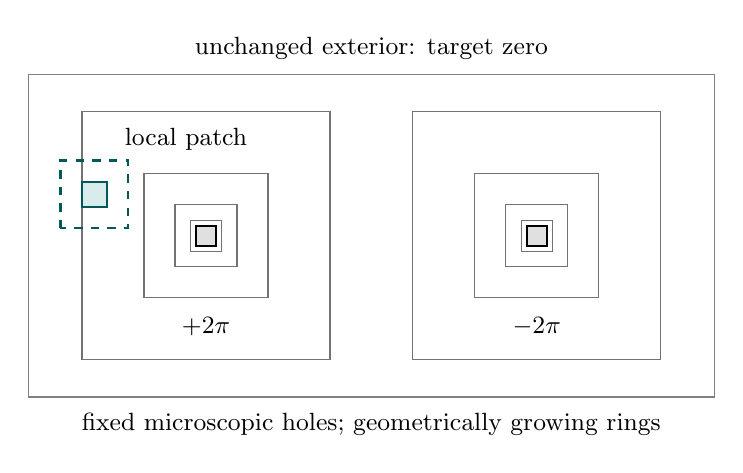
\begin{tikzpicture}[x=1.05cm,y=1.05cm,font=\small]
 \draw[black!50] (-4.15,-1.95) rectangle (4.15,1.95);
 \foreach \x in {-2,2} {
  \foreach \r in {1.5,.75,.375,.1875}
   {\draw[black!55] (\x-\r,-\r) rectangle (\x+\r,\r);}
  \fill[black!12] (\x-.12,-.12) rectangle (\x+.12,.12);
  \draw[thick] (\x-.12,-.12) rectangle (\x+.12,.12);
 }
 \filldraw[fill=teal!15,draw=teal!70!black,thick]
  (-3.5,.35) rectangle (-3.2,.65);
 \draw[teal!70!black,dashed,thick]
  (-3.76,.09) rectangle (-2.94,.91);
 \node[above right] at (-3.1,.91) {local patch};
 \node[fill=white,inner sep=1pt] at (-2,-1.1) {$+2\pi$};
 \node[fill=white,inner sep=1pt] at (2,-1.1) {$-2\pi$};
 \node[above] at (0,2.02) {unchanged exterior: target zero};
 \node[below] at (0,-2.03)
  {fixed microscopic holes; geometrically growing rings};
\end{tikzpicture}
\caption{Schematic geometry for the winding-sector comparison.
Each square ring is partitioned into tiles much smaller than its
distance to the source; only one tile and its enlarged patch are
shown. The construction trims tile junctions and uses collars
with full interfaces. The number of processed tiles is
\(O_M(1+\log n)\), while the unprocessed exterior is kept intact.}
\label{fig:annuli}
\end{figure}


Let \(Z^s,Z^0\) denote the punctured, observation-weighted partition
functions in the shifted and centered sectors. In the same finite
graph let \(Z_{\mathrm g}^s,Z_{\mathrm g}^0\) be the real Gaussian
integrals with gradient precision \(A/a\), the same observations,
outer zero wall, and periods. A free component has a confining
observation, so its constant is integrated rather than fixed.
In comparisons of the two models, a Gaussian pin probability
means the corresponding density at the prescribed coordinates,
or equivalently the common shrinking-neighborhood ratio.
Pin interactions and their determinant formulas are therefore
meaningful although individual Gaussian pin events have
probability zero.

\begin{proposition}[Many-scale sector comparison]
\label{prop:sector-comparison}
For the preceding geometry there are numbers \(\eta_R\to0\) such that,
for each sufficiently large fixed \(R\), one can choose a fixed
\(m_*\) for which
\begin{equation}\label{eq:magnetic-sector-comparison}
 \left|\log\frac{Z^s}{Z^0}
       -\log\frac{Z_{\mathrm g}^s}{Z_{\mathrm g}^0}\right|
       \le C_M(1+\log n)\eta_R.
\end{equation}
For these fixed choices, heights on the two inner rims, in the
bounded cut coordinates just specified, are uniformly tight in
\(n\) and in the outer volume. This is absolute tightness, without
subtracting an additive constant.
\end{proposition}

\subsection{An exact isolation expansion}

Fix an order of the processed tiles. An ordinary step deletes all
still-present bonds from its tile to other tiles, including the
exterior object. Around its core choose a free patch of fixed tile
radius, containing a separating guard and collars wider than any
later support enlargement. In the current local topology, let
\(U_o,U_c\) be the patch before and after this proposed deletion.
Both admit pure-gauge lifts. Replace the bond factor by the scalar
\begin{equation}\label{eq:magnetic-proxy}
 D_i^s=
 \frac{Z_{U_o}^0}{Z_{U_c}^0}
 \frac{Z_{\mathrm g,U_o}^s/Z_{\mathrm g,U_o}^0}
      {Z_{\mathrm g,U_c}^s/Z_{\mathrm g,U_c}^0}
\end{equation}
times the cut factor, plus their difference. In the centered
calculation omit the second fraction, obtaining \(D_i^0\).
For the real Gaussian expansion use its own centered constants
in the same formula.

Selecting the difference marks this step. After a mark, skip every
later step within a fixed number of tile layers, larger than all
patches and guard-testing boxes. Thus marks are separated, their
guard interiors are left untouched, and a subsequently considered
proxy cannot depend on which of the two positive terms is selected
inside a previous difference. This is a finite, exact expansion.
All deviations from the unmarked sequence are supported in bounded
halos of marks. At its end every surviving cross-tile bond, other
than a bond wholly within the exterior, lies in such a halo or
joins it to the exterior.

Normalize each sector by its no-mark term: the product of its
successive proxies and the final isolated tile partition functions,
including the unchanged exterior. For a specified set \(I\) of
\(j\) marks, write \(w(I)\) for its contribution divided by this
normalization.

\begin{lemma}[Pattern gain]\label{lem:magnetic-pattern}
For either model and either sector, after increasing \(m_*\) at
fixed sufficiently large \(R\),
\begin{equation}\label{eq:magnetic-pattern}
                         |w(I)|\le e^{-cRj}.
\end{equation}
Here and below \(c>0\) may decrease, and all fixed constants may
depend on \(b,a,M\), but not on \(n\) or the outer volume.
\end{lemma}

\begin{proof}
We separate the centered normalization, the random guards, and the
local gain.

\paragraph{Conditional differences.}
Prescribe all primary heights \(u_i\) on the guards of the marks.
Let \(K_o,K_c\) be the two positive partition kernels inside one
guard, in the corresponding marked step. Set
\[
 \delta_i(u_i)=
 \frac{|K_o-D_i^sK_c|}{K_o+D_i^sK_c}\le1,
\]
and use \(D_i^0\) in the centered sector. Guard and exterior factors
cancel from this expression. Conditional integration of the product
of differences, followed by the triangle inequality, gives a sum
of at most \(2^j\) positive topologies. In each one the integrand
has the additional factor \(\prod_i\delta_i\). We have not assumed
independence of the random guard data.

\paragraph{Centered normalization.}
For a positive topology \(G\), including its ordinary proxy factors,
its contribution divided by the no-mark term is at most
\begin{equation}\label{eq:magnetic-accounting}
 e^{Cj}\frac{Z_G^s}{Z_G^0}\,
                  \E_{G,s}\prod_i\delta_i.
\end{equation}
Only affected components are included in this display; untouched
final tile factors have been canceled.

Here is the accounting behind \eqref{eq:magnetic-accounting}.
A centered restoration supported in a core lies between its
free-patch value and its value with a separating guard pinned to
zero, whether the actual exterior is absent or present.
Lemma~\ref{lem:comparisons} gives the direction. For a chain
representation, retain the independent chain increments and
restore endpoint matching; all scalar chain normalizers are the
same in these comparisons. A full primary pin on a region \(H\)
containing the restored endpoints makes the restoration a fixed
scalar. Therefore its free-to-guarded multiplicative gap is at
most
\[
 \frac{\Prob(h_p=0\mid h_H=0)}{\Prob(h_p=0)}
                         =e^{D(H,p)}.
\]
Theorems~\ref{thm:pin-interaction} and
\Bcite{an:gaussian-localization} bound this uniformly, and in fact
make its logarithm exponentially small in \(R\) after sufficient
microscopic refinement. Indeed, gradient energy plus cell-average
mass is uniformly coercive in mass-cell units, the clearance is
of order \(R\), and local cell volumes are polynomial in \(R\).
The same cell-cutoff and Hilbert--Schmidt estimates apply to the
bounded rectangular shapes here, including at free walls.

Only \(O_M(j)\) such normalization comparisons are charged.
Take a union containing sufficiently enlarged halos of all marks,
with a further collar beyond every skip and dependence radius.
Telescope separately the actual centered partition functions along
the positive branch and along the no-mark branch in this union.
Include the whole exterior object and its neighboring collar if
surviving bonds or changes can meet it. Count every event in the
union, including one clipped at its artificial boundary. At a
clipped event use the proxy clipped in the same manner on both
paths. Before every boundary event, the two histories agree
on its entire proxy patch: the collar contains every affected
or skipped step and exceeds the proxy's dependence radius.
Thus the scalar change from an original proxy to its clipped
version is identical on both paths and cancels. There are
\(O_M(j)\) events; the exterior itself
has none. Final integrals and proxies outside the affected region
also cancel, while the initial centered integrals on the two paths
are identical. Each remaining true-to-proxy ratio is bounded by
the preceding centered sandwich. Enlarging by whole tile layers
ensures that clipped comparisons still have separating guards
with unchanged clearance. Artificial point contacts add no bonds.
More explicitly, call this induced union \(U\), with free
artificial walls, and let \(\alpha\) be either deletion history.
For an actual deletion \(e\), put
\[
 T_e^\alpha=\frac{Z_{U,e\text{ before}}^0}
                  {Z_{U,e\text{ after}}^0},
 \qquad \widetilde D_e^\alpha
       =\text{its centered proxy clipped to }U.
\]
A skipped step or an open marked choice is not a deletion;
a cut marked choice is a deletion and carries its proxy.
The exact telescoping identity is
\begin{equation}\label{eq:magnetic-centered-telescope}
 Z_{U,\mathrm{final}\,\alpha}^0
       \prod_{e\in\alpha}\widetilde D_e^\alpha
   =Z_{U,\mathrm{initial}}^0
       \prod_{e\in\alpha}\frac{\widetilde D_e^\alpha}{T_e^\alpha}.
\end{equation}
The initial integral is common to both histories. In their
quotient, changing an original proxy to a clipped one cancels
at the artificial boundary, where the histories agree through
a collar wider than the proxy radius. Final components outside
\(U\) are identical and have no surviving bond to \(U\);
including an attached exterior object ensures this also for
terminal connections. Each product on the right has \(O_M(j)\)
factors, each bounded with its inverse by the centered
sandwich, also up to a new free wall. An exterior object has
no deletion events, and its whole inner collar has only
\(O_M(1)\) tiles. Thus its arbitrarily large microscopic
volume adds no charge. This proves \(e^{Cj}\) without an
error proportional to untouched tiles, as in
\Bcite{en:normalization}.

The shifted proxy factors agree off the same halos. Within them
each Gaussian shifted minimum energy is bounded by a fixed
constant: try the local target lift, whose gradient energy is
bounded and whose observation error is zero. Likewise, each
isolated regular tile has shifted-to-centered ratio bounded
below by a fixed positive constant after refinement.
Theorem~\ref{thm:mixed-limits}, including summation of constants
and the uniform fractional mean, gives convergence to its
Gaussian ratio; the same target trial bounds its Gaussian energy.
These constants are uniform for large \(R\) once the microscopic
mesh has been chosen. The exterior alone is unshifted.
These facts give the remaining shift accounting in
\eqref{eq:magnetic-accounting}, even when an affected connected
component has no global lift.

\paragraph{Cutting with prescribed guards.}
Cut disjoint larger boxes of tiles around the marks, well outside
their guards. For joint partition weights \(J_G(s,u)\), normalized
at centered shifts and zero prescribed guard data, affine
comparison gives
\begin{equation}\label{eq:magnetic-guard-cut}
 \frac{J_G(s,u)}{J_G(0,0)}
       \le
 \frac{J_{G^{\rm cut}}(s,u)}{J_{G^{\rm cut}}(0,0)}.
\end{equation}
This includes the connection, observation shifts, and prescribed
primary heights as affine coordinates. Restoring the cut bonds
is an increase of precision, so Lemma~\ref{lem:comparisons}
applies. This is the comparison of \Bcite{en:shifted-box}, now
using the established Skellam comparison.

To return from zero prescribed data to unprescribed data, the
remaining centered factor is a ratio of probabilities that all
these guards are zero. Impose them successively. For each guard
use a still larger separating patch, disjoint from the cuts and
the previously imposed guards. Its centered pin probability in
the full and clipped graphs lies between common open-patch and
outer-pinned values, whose ratio is bounded by a separated
hard-pin interaction. Their product costs at most \(e^{Cj}\).
Skip distances were chosen large enough to keep these boxes
disjoint.

We may enlarge the affected region in
\eqref{eq:magnetic-accounting} to include every otherwise
untouched isolated tile in these boxes; their shifted ratios
cost at most another \(e^{Cj}\). Include the exterior object
whenever it is met. Sum \eqref{eq:magnetic-guard-cut} over the
data, keeping the same \(\delta_i\), since cutting beyond a
guard does not change its interior kernel. The outside
shifted-to-centered factor is at most one. Inside, the cut
boxes are independent and their own shifted-to-centered
factors are also at most one. All twists within a box are now
ordinary bounded observation shifts after integer gauge changes.
It remains to prove, in either of its two positive topologies,
\begin{equation}\label{eq:magnetic-local-gain}
                     \E_{{\rm box},s}\delta_i\le e^{-cR}.
\end{equation}

\paragraph{The local gain at typical data.}
Write \(K_t(y,u)\), \(t=o,c\), in a common bounded lift,
where \(y=Bv\), and cancel factors depending only on the guard
or its exterior. Put
\[
 R(u)=\frac{K_o(0,u)}{K_c(0,u)},\qquad
 r_\Delta(u)=\frac{R(u)}{R(0)},\qquad
 F_t(y,u)=\log\E_{t,0}(e^{\ip{y}{Bh}}\mid h_p=u).
\]
The common observation constant \(e^{-\norm y^2/2}\)
cancels as well. If
\[
 P_{\mathrm g}(y)=
 \log\frac{Z_{\mathrm g,U_o}(y)/Z_{\mathrm g,U_o}(0)}
           {Z_{\mathrm g,U_c}(y)/Z_{\mathrm g,U_c}(0)},
\]
the exact decomposition is
\begin{equation}\label{eq:magnetic-kernel-decomposition}
 \log\frac{K_o(y,u)}{D_i^sK_c(y,u)}
   =\log\frac{R(0)}{D_i^0}+\log r_\Delta(u)
       +F_o(y,u)-F_c(y,u)-P_{\mathrm g}(y).
\end{equation}
The first term is \(O(e^{-cR})\) in the refinement limit
by the centered sandwich. The full-core pin ratio \(r_H\)
of the \emph{cut centered law} satisfies
\(\log r_H\le\log r_\Delta\le0\), with \(H\) containing
the restored bonds. No separate scaling limit for
\(r_\Delta\) is required: this sandwich and the bounded
discrepancy \(\delta_i\) suffice.

Theorems~\ref{thm:mixed-limits} and~\ref{thm:pin-interaction}
give joint convergence of \(r_H\) and the conditional Laplace
terms in the finite-observation sense, at this fixed geometry.
They apply under the centered or tilted laws of either
topology. One can first analyze conditioning in the whole cut
box: its interior kernel given the full guard agrees with that
in any completion with the same interior and guard. Transfer
between cut and restored typical data follows explicitly as
follows. For their centered guard laws \(\mu_p,\nu_p\),
Lemma~\ref{lem:restoration} gives
\[
 r_H\le \frac{\dd\nu_p}{\dd\mu_p}\le e^{D(H,p)}.
\]
Thus \(\mu_p(E)\to0\) implies \(\nu_p(E)\to0\), and
\[
 \mu_p(E)\le \mu_p(r_H\le\kappa)+\kappa^{-1}\nu_p(E).
\]
Strict positivity of the limiting Gaussian \(r_H\), followed
by \(\kappa\downarrow0\), gives the converse. Taking a common
finite list of probes therefore makes both conditional
Laplace approximations and the pin-ratio approximation joint
under either law. Uniform fixed-tilt exponential moments
transfer exceptional sets to either tilted law by H\"older.
Probe exhaustion is after refinement at this fixed geometry.
Nothing here asserts a limit uniform at arbitrary microscopic
guard values.

For completeness, the quantitative Gaussian calculation is as
follows. Let \(u_c\) be the cut harmonic prediction from the guard
in the centered massive energy, and let \(\chi\) equal one on
the core and vanish before the guard. With \(T\) denoting the
gradient-plus-observation energy and \(y=Bv\), Gaussian
localization gives
\begin{equation}\label{eq:magnetic-prediction}
 \E\norm{\chi u_c}_T^2
       \le {\rm poly}(R)e^{-cR}(1+\norm y^2).
\end{equation}
This is the localized-operator and Hilbert--Schmidt estimate in
\Bcite{an:gaussian-localization}, or \Bcite{en:prediction}.
Restoration decreases centered guard covariance, and the
deterministic prediction due to the tilt is bounded by the
same localized operator. The Gaussian full-core pin ratio
satisfies
\[
                  -2\log r_H^{\mathrm g}
                         \le \norm{\chi u_c}_T^2.
\]
Indeed, subtracting this cutoff prediction makes the
conditional mean zero on the core without changing its guard
values. Orthogonal projection onto the restored admissible
space also bounds the change of prediction between cut and
restored topologies by \(\norm{\chi u_c}_T\). This remains
valid when restoration matches two previously free traces:
vanishing on the core is an admissible correction.
Thus the linear-in-data part of the conditional Laplace
discrepancy is bounded by \(C\norm y\norm{\chi u_c}_T\).
In fact, for \(f=B^*y\), centered Gaussian conditional means
\(m_t\), and conditional covariances \(C_t^p\),
\[
 F_o(y,u)-F_c(y,u)
  =\ip{f}{m_o(u)-m_c(u)}
       +\frac12\ip{f}{(C_o^p-C_c^p)f}.
\]
Here \(u_c=m_c(u)\) is always the cut-law prediction,
evaluated under either topology's data, and
\(\norm{f}_{T^*}\le\norm y\).

The conditional quadratic discrepancy from the open-patch
comparison is at most
\[
                    {\rm poly}(R)e^{-cR}\norm y^2.
\]
One way to see all of its
locality requirements is to compare the changes of the
minimized observation-energy matrices under restoration,
with and without the zero guard pin. Each change decays
exponentially as an observation index recedes from the core,
by positivity of the added form and a localized trial cut
off near restored edges. Near the core, the guard pin's
own effect decays from the guard. Cross entries follow
by positive-form Cauchy--Schwarz. The same argument at
the patch boundary compares the open patch with the full
box. There are only polynomially many entries; guard-only
and exterior terms cancel from the kernel ratio.
Finite guard probes can be exhausted after these estimates.
This is the projection argument underlying \Bcite{en:good-box}.

Here \(\norm y\le{\rm poly}(R)\), so all these bounds have an
exponentially small right side after weakening \(c\).
Use
\[
 \left|\frac{x-1}{x+1}\right|
                       \le\min\{1,|\log x|\},\qquad x>0.
\]
Convergence in probability of the finite-observation
approximations, the bound \(\delta_i\le1\), and Gaussian
localization prove \eqref{eq:magnetic-local-gain}, with slack.
At fixed \(R\), increase \(m_*\) so it holds uniformly over
the finite geometries and compact target families. Applying
it in the disjoint boxes, absorbing the factors \(2^j e^{Cj}\),
proves \eqref{eq:magnetic-pattern}.
\end{proof}

\subsection{Factorization, logarithmic errors, and rim insertions}

The pattern bound alone must be supplemented by exact dependence
information. Enlarge each mark halo past all skip and proxy radii,
and join two potential marks if their enlarged halos meet or
if they can attach to the same exterior terminal node. This
defines a graph of bounded degree, independent of \(R,n,L\).
For disconnected groups of marks the normalized weights factor.
Indeed, a skip depends only on nearby earlier marks, a considered
proxy only on the current cuts in its patch, and an unmarked
deletion isolates its tile. All final non-product integrals lie
inside halos, possibly attached to the exterior. Distinct groups
have disjoint variables and no surviving bonds between them.
If the exterior could connect them, they were joined through its
terminal node. The signed sums over final positive topologies
therefore factor as well, with the original global order merely
restricted to each group. All untouched factors cancel exactly.
Violations of the skip rule have weight zero, a condition
checked separately in each component.

Consequently the normalized partition is a finite gas of
compatible connected mark sets, with activities bounded by
\(e^{-cRj}\) for size \(j\). We record explicitly the smallness
argument for signed activities. In a graph of bounded degree,
there are at most \(D^j\) connected sets of size \(j\) containing
a given site, and their closed neighborhoods have at most
\(D'j\) sites. Let \(\Xi(V)\) be the gas partition sum when marks
are allowed only in a set \(V\); ordinary unmarked steps are
still retained. Removing one allowed site \(x\) and summing
over the connected polymer containing it gives
\[
 \frac{\Xi(V)}{\Xi(V\setminus\{x\})}-1
  =\sum_{\substack{P\ni x\\P\subset V}}
       w(P)\,
       \frac{\Xi(V\setminus N[P])}
            {\Xi(V\setminus\{x\})}.
\]
Induct on \(|V|\). If smaller deletion ratios lie in
\([1-\eps_R,1+\eps_R]\), the absolute value of the right side
is at most
\[
       \sum_{j\ge1}D^j e^{-cRj}(1-\eps_R)^{-D'j}.
\]
For sufficiently large \(R\), this is at most
\(\eps_R=O(e^{-c'R})<1/2\), after adjusting constants.
The induction gives nonvanishing and positivity, also for all
restricted sums, and
\begin{equation}\label{eq:magnetic-gas-log}
                         |\log\Xi(V)|\le 2\eps_R|V|.
\end{equation}
Thus signed cancellations cannot invalidate the logarithmic
estimate.

The shifted-to-centered ratios of corresponding no-mark proxies
are identical in the lattice and Gaussian models, by
\eqref{eq:magnetic-proxy}. For final isolated tiles their ratios
have arbitrarily small logarithmic discrepancies after refinement,
by Theorem~\ref{thm:mixed-limits} and the uniform fractional mean
in Theorem~\ref{thm:coefficient-gap}. Their Gaussian energies are
uniformly bounded by trying the target; hence the limiting
ratios are bounded away from zero. The isolated exterior has
ratio one. Apply \eqref{eq:magnetic-gas-log} to the two sectors
of both models. Since there are at most \(C_M(1+\log n)\)
processed tiles, this proves
\eqref{eq:magnetic-sector-comparison}, choosing all local
refinement errors smaller than a prescribed quantity tending
to zero with \(R\).

We next prove the tightness assertion of
Proposition~\ref{prop:sector-comparison}. For a primary inner-rim
site \(x\), insert \(e^{h_x}\) or \(e^{-h_x}\) in its bounded
cut coordinates. The microscopic volume of every fixed-radius
patch near \(x\) is bounded in terms of \(m_*,R,M\), also for
the rim translated to the other source. Add one distinguished
item at its tile in the preceding expansion. Discard difference
gains in a fixed neighborhood of this item; if an insertion
lies in a marked kernel, first bound the absolute difference
by the sum of its positive terms.

Clip a separate box about the distinguished item, including
all necessary neighboring tiles, while retaining disjoint
comparison boxes for more distant marks. Only boundedly many
ordinary gains have been discarded. The prescribed-guard
cutting inequality remains valid with the fixed real linear
tilt \(\pm h_x\) in the numerator, by
Lemma~\ref{lem:comparisons}. This uses monotonicity of the
tilted ratio, not the bound one for it. In the distinguished
box the ratio with the insertion is bounded by a finite
constant: each component has confining average penalties,
there are boundedly many lattice sites, the edge sums have
all fixed exponential moments, and translation sums are
Gaussian-confined. This constant may depend arbitrarily on
the fixed \(m_*,R,M\).
The inserted functional remains literally \(\pm h_x\)
throughout this comparison, not an extension by a flow or a
harmonic prediction. After cutting it is supported entirely
in the distinguished box. No matching constraint remains
to its exterior, so every other factor is untilted and has
shifted-to-centered ratio at most one. A bounded change of
chart contributes only a bounded scalar. The rounded
distinguished graphs form a finite set at fixed \(m_*\),
and their target vectors form compact sets, making the
finite insertion constant uniform for all integer \(n\).

The previous centered accounting applies with the distinguished
halo included. Connected weights containing the distinguished
item are therefore bounded by
\[
                       C_{m_*,R,M}e^{-cRj},
\]
where \(j\) is the number of ordinary marks; the bounded
number of lost gains is absorbed in the constant. All other
components factor as before. More explicitly, let \(*\) be
the forced distinguished item and let \(\Xi\) be the gas
without the insertion. Group the inserted expansion by the
connected component containing \(*\). With \(P\subset V\)
its ordinary marks, the exact normalized expression is
\[
 \E_s e^{\pm h_x}
   =\sum_{\substack{P\subset V\\P\cup\{*\}\ \mathrm{connected}}}
       W_*(P)\,
       \frac{\Xi(V\setminus N[P\cup\{*\}])}{\Xi(V)}.
\]
The weights include the finitely many altered factors in
the distinguished halo. For \(j=|P|\), their absolute values
are at most \(C_{m_*,R,M}e^{-cRj}\), the number of connected
choices is at most \(D^{j+1}\), and the removed neighborhood
has at most \(D'(j+1)\) sites. The deletion bounds proving
\eqref{eq:magnetic-gas-log} therefore dominate this expression
by
\[
 C_{m_*,R,M}
   \sum_{j\ge0}D^{j+1}e^{-cRj}
                    (1-\eps_R)^{-D'(j+1)}<\infty.
\]
This bound is independent of \(|V|\); no extensive
log-partition bound is used when dividing the two sums.
Consequently,
\begin{equation}\label{eq:magnetic-rim-moment}
       \E_s e^{h_x}+\E_s e^{-h_x}\le C_{m_*,R,M},
\end{equation}
uniformly in \(n,L\). There are boundedly many inner-rim sites
for fixed \(m_*\), so \eqref{eq:magnetic-rim-moment} proves
the asserted absolute tightness and completes the proof of
Proposition~\ref{prop:sector-comparison}.

\subsection{Filling the holes and the angular energy}

Return to the full dual partition of Lemma~\ref{lem:duality}.
First add the observation penalties, only outside the holes;
this lowers its shifted-to-centered ratio. Compare this
weighted full partition with its punctured version. With
normalized edge weights \(p_b\), the centered filling kernel
is bounded above by one: retain a spanning forest attaching
the finitely many removed vertices to their rim, sum the
forest increments using \(\sum_jp_b(j)=1\), and bound the
other edge factors by one. A fixed harmless normalization
convention would instead give a fixed upper bound.

By Proposition~\ref{prop:sector-comparison}, in the shifted
punctured law all adjacent rim values are bounded by a
fixed constant with uniformly positive probability.
Fill both holes with any fixed bounded configuration in
the cut coordinates. There are only finitely many required
integer differences, bounded in terms of the fixed choices,
including those on the continued offset path. All their
weights \(p_b(j)\) are strictly positive. Thus the numerator
filling factor is bounded below on this event by a positive
constant. We obtain
\begin{equation}\label{eq:magnetic-fill}
 \E_{\mu_{L,b}}\cos(\theta_0-\theta_{ne_1})
                         \ge c_{m_*,R,M,b}\frac{Z^s}{Z^0}
\end{equation}
uniformly for the large outer boxes under consideration.
The exterior dual face remains fixed at zero throughout,
which is the original free spin boundary condition; no
primal boundary spin has been fixed.

For the real Gaussian model, completing the square gives
the shifted-to-centered ratio as the exponential of minus
one half the minimum affine energy. Trying the sampled
target \(v\) makes the observation error zero and matches
the exterior pin. Therefore
\begin{equation}\label{eq:magnetic-energy}
 -\log\frac{Z_{\mathrm g}^s}{Z_{\mathrm g}^0}
       \le \frac1{2a}\bigl(4\pi\log n+O_{m_*}(1)\bigr).
\end{equation}
Indeed, near each source the angular energy is
\[
 \int_{m_*/n<|z|<c}|\nabla\arg z|^2\,\dd z
                        =2\pi\log n+O_{m_*}(1).
\]
Replacing the circular inner boundary by a square changes
only the bounded term. The other angle and the cutoff
corrections are smooth near that source; their cross terms
with its \(1/|z|\) gradient are integrable. All remaining
energies are bounded. On the lattice, derivative errors
of order \(r^{-2}\) at distance \(r\) give summable errors
in the squared-gradient sum. Thus the two singularities
give exactly \(4\pi\), with no extra factor from oriented
edge counting.

\begin{proof}[Proof of Proposition~\ref{prop:spin-lower}]
Choose \(M\), then arbitrarily large fixed \(R\), and then
sufficiently large fixed \(m_*\) as in
Proposition~\ref{prop:sector-comparison}. Combining
\eqref{eq:magnetic-sector-comparison},
\eqref{eq:magnetic-fill}, and \eqref{eq:magnetic-energy}
gives, uniformly in sufficiently distant outer boundaries,
\[
 \log \E_{\mu_{L,b}}\cos(\theta_0-\theta_{ne_1})
 \ge -\frac{2\pi}{a}\log n
       -C_M(1+\log n)\eta_R-O_{m_*,R,M,b}(1).
\]
For each fixed \(n\), first take the prescribed free-box
limit \(L\to\infty\). Divide by \(\log n\), and then
take the liminf as \(n\to\infty\). All hole and insertion
constants were fixed before this limit and disappear.
Finally let \(R\to\infty\), obtaining the claimed lower
exponent. Since \(0<C_b(n)\le1\), this polynomial lower
bound also implies \(m(b)=0\).
\end{proof}
